%%%%%%%%%%%%%%%%%%%%%%%%%%%%%%%%%%%%%%%%%%%%%%%%%%%%%%%%%%%%%%%%%%%%%%
% Universidade Federal de Santa Catarina             
% Biblioteca Universitária                     
%----------------------------------------------------------------------
% Exemplo de utiliza\c{c}\~ao da documentclass ufscThesis
%----------------------------------------------------------------------
% (c)2013 Roberto Simoni (roberto.emc@gmail.com)
%         Carlos R Rocha (cticarlo@gmail.com)
%         Rafael M Casali (rafaelmcasali@yahoo.com.br)
%%%%%%%%%%%%%%%%%%%%%%%%%%%%%%%%%%%%%%%%%%%%%%%%%%%%%%%%%%%%%%%%%%%%%%%
\documentclass{ufscThesis} % Definicao do documentclass ufscThesis	

%----------------------------------------------------------------------
% Pacotes usados especificamente neste documento
\usepackage{graphicx}
\usepackage{color}
\usepackage{listings}
\usepackage{pgfgantt}
\usepackage{enumitem}
\usepackage{amsmath}
\usepackage{paralist}
\usepackage{booktabs}
\usepackage[T1]{fontenc}
\usepackage{inconsolata}

%----------------------------------------------------------------------
% Comandos criados pelo usuário
\newcommand{\afazer}[1]{{\color{red}{#1}}} % Para destacar uma parte a ser trabalhada

%----------------------------------------------------------------------
% Identificadores do trabalho
% Usados para preencher os elementos pré-textuais
\instituicao[a]{Universidade Federal de Santa Catarina} % Opcional
\departamento[a]{Departamento de Inform\'atica e Estat\'istica}
\grau{Bacharel em Ci\^encias da Computa\c{c}\~ao}
\curso[o]{Ci\^encias da Computa\c{c}\~ao}
\documento[o]{Trabalho de conclus\~ao de curso} % [o] para disserta\c{C}ão [a] para tese
\titulo{Implementa\c{c}\~ao de um gateway CoAP/GPRS para servi\c{c}os de monitoramento em redes de sensores sem fio}
\autor{Rafael de Lucena Valle}
\local{Florian\'opolis} % Opcional (Florianópolis é o padrão)
\data{15}{maio}{2014}
\orientador[Orientador]{Prof. Dr. Ant\^onio Augusto Fr\"ohlich}
\coorientador[Coorientador]{Prof. M.Sc. Arliones Hoeller Jr}
\coordenador[Coordenador]{Prof. Dr. Vit\'orio Mazzola}

\numerodemembrosnabanca{3} % Isso decide se haverá uma folha adicional
\orientadornabanca{sim} % Se faz parte da banca definir como sim
\coorientadornabanca{nao} % Se faz parte da banca definir como sim
\bancaMembroA{Prof. Dr. Ant\^onio Augusto Fr\"ohlich} %Nome do presidente da banca
\bancaMembroB{Prof. Dr. Eng. Rafael Luiz Cancian} % Nome do membro da Banca
\bancaMembroC{Prof. Dr. Frank Siqueira} % Nome do membro da Banca

\agradecimento{Inserir os agradecimentos aos colaboradores \'a execu\c{c}\~ao do trabalho.}

\textoResumo {  Redes de sensores e atuadores s\~ao utilizadas para a captura, processamento de informa\c{c}\~ao e\
    para atua\c{c}\~ao sobre um ambiente, tornando-as importantes em aplica\c{c}\~oes de controle, telemetria\
    e rastreamento.
    
    Estas redes s\~ao compostas por n\'os sensores que os trabalham em conjunto afim obter dados de um ambiente.\
    Possuem processadores, transmissores e receptores simplificados, restri\c{c}\~oes de mem\'oria e energia,\
    geralmente sem alimenta\c{c}\~ao constante de energia.\
    Contudo possuem um custo baixo de equipamentos, tornando interessante a implanta\c{c}\~ao destes sistemas.
    
    O protocolo HTTP, um protocolo de aplica\c{c}\~ao muito utilizado na atualidade, foi desenvolvido para computadores\
    de prop\'osito geral, onde essas restri\c{c}\~oes n\~ao existem. Um protocolo leve como CoAP pode tornar vi\'avel\
    o desenvolvimento de aplica\c{c}\~oes web em redes de sensores sem fio.

    Este trabalho prop\~oe uma infraestrutura de comunica\c{c}\~ao entre redes de sensores sem fio e a Internet,\
utilizando protocolos leves entre os n\'os sensores e um gateway GPRS para aproveitar a cobertura da tecnologia GPRS.

    Com a implementa\c{c}\~ao do CoAP \'e esperado uma redu\c{c}\~ao de consumo de energia e mem\'oria,\
    em rela\c{c}\~ao a outros protocolos de aplica\c{c}\~ao existentes.}

\palavrasChave{ internetworking WSN IPv6 GPRS CoAP IoT}

%----------------------------------------------------------------------
% Início do documento                                
\begin{document}
%--------------------------------------------------------
% Elementos pré-textuais
\capa
%\folhaderosto%[comficha] % Se nao quiser imprimir a ficha, é só não usar o parâmetro
%\folhaaprovacao
%\paginadedicatoria
%\paginaagradecimento
%\paginaepigrafe

\paginaresumo
%\paginaabstract
%\pretextuais % Substitui todos os elementos pre-textuais acima
\listadefiguras % as listas dependem da necessidade do usuário
%\listadetabelas
\abreviatura{CoAP}{Constrained Aplication Protocol}
\abreviatura{EPOS}{Embedded Parallel Operating System}
\abreviatura{HTTP}{Hipertext Transfer protocol}
\abreviatura{IETF}{Internet Engineering Task Force}
\abreviatura{M2M}{Machine-to-Machine}
\abreviatura{REST}{Representatational State Transfer}
\abreviatura{UDP}{User Datagram Protocol}
\abreviatura{IoT}{Internet of Things}
\abreviatura{JSON}{JavaScript Object Notation}
\abreviatura{XML}{Extensible Markup Language}
\abreviatura{ADESD}{Application Driven Embedded System Design}
\abreviatura{SOC}{Service-Oriented Computing}

\listadeabreviaturas

%\listadesimbolos
\sumario
%--------------------------------------------------------
% Elementos textuais

\chapter{Introdu\c{c}\~ao}
Redes de sensores e atuadores s\~ao utilizadas para a capta\c{c}\~ao, processamento de informa\c{c}\~ao e atua\c{c}\~ao sobre um ambiente, tornando-as importantes em aplica\c{c}\~oes de controle, telemetria e rastreamento de sistemas.

N\'os que participam destas redes geralmente s\~ao compostos por computadores e r\'adios simplificados, que possuem restri\c{c}\~oes de mem\'oria, processamento, energia e capacidade de comunica\c{c}\~ao, mas um custo relativamente baixo de equipamentos.

O maior consumo de energia neste tipo de aplica\c{c}\~ao \'e do r\'adio, portanto o desafio dos algoritmos de comunica\c{c}\~ao nesta \'area \'e manter os r\'adios ligados o m\'inimo de tempo poss\'ivel sem comprometer a conectividade do n\'o.

\section{Objetivos}
O objetivo geral desse trabalho \'e descrever e implementar webservices em uma rede sensores sem fio que far\~ao a aquisi\c{c}\~ao dos dados do ambiente e disponibilizar\~ao as informa\c{c}\~oes captadas na Internet.

\subsection{Objetivos Espec\'ificos}
Este trabalho realizar\'a o desenvolvimento de aplica\c{c}\~oes web e software de sistema para fazer a ponte entre a rede de sensores e a Internet. O Sistema operacional utilizado ser\'a o EPOS, que possui uma implementa\c{c}\~ao de pilha UDP/IP. A aplica\c{c}\~ao integradora GPRS/802.15.4 ir\'a executar na plataforma EposMoteII utilizando uma extens\~ao GPRS.

A comunica\c{c}\~ao entre os n\'os da rede ser\'a feita atrav\'es do protocolo de aplica\c{c}\~ao CoAP, um protocolo espec\'ifico para redes de sensores sem fio. Ser\'a utilizado um porte de uma implementa\c{c}\~ao livre do protocolo CoAP.

Sendo assim, os objetivos espec\'ificos s\~ao:

\begin{enumerate}
    \item{Portar o protocolo CoAP para o EPOS;}
    \item{Implementar uma aplica\c{c}\~ao para redes de sensores sem fio;}
    \item{Desenvolver a aplica\c{c}\~ao gateway GPRS/802.15.4.}
    \item{Desenvolver uma aplica\c{c}\~ao web para visualiza\c{c}\~ao da informa\c{c}\~ao;}
    \item{Avaliar a soluc\c{c}\~ao desenvolvida.}
\end{enumerate}

\section{Justificativa}

Os mecanismos de confiabilidade na transmiss\~ao de dados, t\'ecnicas para se manter uma conex\~ao do TCP e rearranjos que s\~ao feitos para garantir a ordem das mensagens recebidas n\~ao s\~ao adequados para um dispositivos com suprimento limitado de energia, como uma bateria ou uma placa fotovolt\'aica. Estas t\'ecnicas fazem que os transmissores fiquem ligados por mais tempo, para manter a conex\~ao ou at\'e mesmo para reenvio de mensagens.

O maior consumo de energia de um n\'o sensor \'e no envio e recebimento de dados, quando mantem seu transmissor ligado. Al\'em disso quem recebe a mensagem precisa mont\'a-la e tratar as partes corrompidas, podendo gerar retransmiss\~oes.

Por sua vez o protocolo do UDP, n\~ao mant\'em conex\~ao, dados s\~ao recebidos fora de ordem e o envio \'e feito de uma mensagem por vez. Isto implica tamb\'em na redu\c{c}\~ao do tamanho do cabe\c{c}alho do pacote.

Estas caracter\'isticas demostram uma alternativa interessante para estes equipamentos limitados. Testes feitos em implementa\c{c}\~oes de sistemas operacionais similares ao EPOS, como Contiki e TinyOS, utilizando o protocolo CoAP demonstram redu\c{c}\~ao no consumo de energia e mem\'oria em rela\c{c}\~ao ao HTTP \cite{transportApp}.

A falta de padroniza\c{c}\~ao dos protocolos afeta o desenvolvimento de uma rede p\'ublica ub\'iqua de uma cidade inteligente, por exemplo. Grande parte das solu\c{c}\~oes utiliza protocolos propriet\'arios que se comunicacam apenas com os produtos de um mesmo fabricante.

O protocolo HTTP foi desenvolvido para comunica\c{c}\~ao de computadores de prop\'osito geral, onde as restri\c{c}\~oes citadas n\~ao s\~ao comuns. Em rela\c{c}\~ao ao tamanho, o pacote HTTP \'e um problema para redes 802.15.4, j\'a que estas redes possuem uma restri\c{c}\~ao de 128 bytes em sua PDU. O protocolo TCP precisa transmitir mensagens adicionais para manter uma conex\~ao, outra caracter\'istica que n\~ao \'e interessante para RSSF.

Um protocolo leve como CoAP pode tornar vi\'avel a cria\c{c}\~ao de aplica\-\c{c}\~oes web em redes de sensores sem fio por um baixo custo. Neste trabalho \'e proposto uma infraestrutura de comunica\c{c}\~ao entre redes de sensores sem fio e a Internet, utilizando protocolos leves entre os n\'os sensores e um gateway GPRS para \'areas sem acesso \`a WIFI, aproveitando a vasta abrang\^encia da tecnologia de telefonia. Com a utiliza\c{c}\~ao do CoAP \'e esperado uma redu\c{c}\~ao de consumo de energia e mem\'oria, em rela\c{c}\~ao a outros protocolos de aplica\c{c}\~ao existentes.

Em lugares aonde n\~ao existe o acesso a rede cabeada ou sem fio, como lugares afastados, na \'area rural, por exemplo a distribui\c{c}\~ao da informa\c{c}\~ao para Internet ser\'a feita atrav\'es de um gateway.

O gateway ser\'a composto por um EposMoteII e um m\'odulo GPRS, respons\'avel por fazer a ponte entre a rede de sensores e a Internet. Atualmente o padr\~ao GPRS oferece a maior cobertura dentre as tecnologias de transmiss\~ao de telefonia no Brasil, atingindo cerca de 5477 munic\'ipios.\cite{coberturaGPRS}


\section{Metodologia}

Ser\'a feito um levantamento dos componentes de software e hardware necess\'arios para o desenvolvimento do gateway 802.15.4/GPRS. Neste caso utilizando o mote EPOSMote II e um m\'odulo GPRS, que ser\'a desenvolvido em paralelo a implementa\c{c}\~ao do protocolo de aplica\c{c}\~ao CoAP no sistema operacional EPOS.

Durante o desenvolvimento do protocolo, testes ser\~ao executados para verificar o correto comportamento e diminuir a depura\c{c}\~ao em hardware, que geralmente leva mais tempo.

Nos testes de integra\c{c}\~ao do gateway, ser\'a utilizada uma placa de desenvolvimento em conjunto com um m\'odulo M95 da Quectel disponibilizada pelo LISHA. Ser\~ao realizads testes de envio de mensagens em diversos protocolos, inclusive testes com comandos propriet\'arios adicionais do modem.

Para testes de integra\c{c}\~ao, as aplica\c{c}\~oes ser\~ao executadas na plataforma de sensores sem fio EPOS Mote II utilizando o EPOS com o CoAP desenvolvido.


\chapter{Revis\~ao Bibliografica}
As t\'ecnologias de ambientes inteligentes est\~ao est\~ao sendo desenvolvidas e ser\~ao um grande passo para as \'areas como: constru\c{c}\~ao civil, industria, transporte e automa\c{c}\~ao residencial.

Para agirem de forma inteligente, estes ambientes necessitam de informac\c{c}\~ao sobre o contexto aonde ser\~ao implantados. As redes de sensores sem fio s\~ao um componente chave para estes ambientes, adquirem este contexto captando e comunicando os dados do ambiente.\cite{lewis2004wireless}

Este cap\'itulo apresenta uma vis\~ao geral sobre redes de sensores sem fio, arquitetura orientada a servi\c{c}os e os protocolos de aplica\c{c}ao existentes.

\section{Redes de sensores sem fio}

O desenvolvimento destas redes foi inicialmente motivada por aplica\c{c}\~oes militares e hoje s\~ao utilizados em 
utilizados em diversas aplica\c{c}\~oes na ind\'ustria, no monitoramento e controle de processos industriais, supervis\~ao de maquinas, monitoramento de ambientes, estruturas e tubula\c{c}\~oes, autom\c{c}\~ao resid\^encial, coleta de dados de pacientes, entre outros.

Avan\c{c}os recentes nas tecnologias de sistemas eletr\^onicos, semicondutores, sensores, microcontroladores e r\'adios tornaram poss\'ivel o desenvolvimento de redes de sensores de baixo custo e baixo consumo uma realidade.

Os requisitos para uma rede de sensores distribu\'ida s\~ao: reconfigura\c{c}\~ao com esta\c{c}\~ao base, controle auton\^omo de opera\c{c}\~ao e ger\^encia de energia, auto-monitoramento, efici\^encia energ\'etica para longo tempo de opera\c{c}\~ao e apta a incorporar diversos sensores.\cite{542724}


Geralmente tais redes possuem centenas ou milhares de n\'os sensores e possuem as seguintes caracter\'isticas: pouca mem\'oria, pouco alcance do r\'adio, baixa capacidade de processamento e bateria, e custo reduzido. Comunicam-se entre si e com esta\c{c}\~oes base utilizando seus r\'adios sem fio, permitindo dissemina\c{c}\~ao da informa\c{c}\~ao para processamento remoto, visualiza\c{c}\~ao, an\'alise e armazenamento. A figura \ref{wsnOverview} d\'a uma vis\~ao geral sobre a comunica\c{c}\~ao destes n\'os.

\begin{figure}[H]
   \label{wsnOverview}
   \centering
   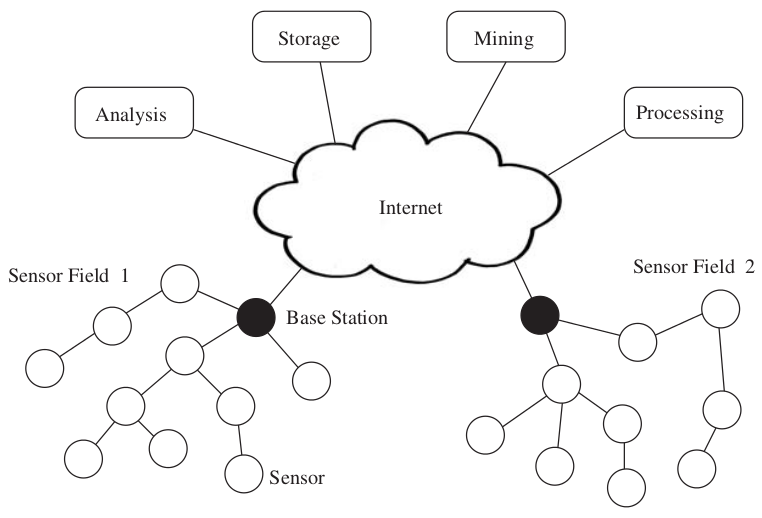
\includegraphics[width=0.8\textwidth]{figuras/wsn.png}
   \caption{\cite{dargie2010fundamentals}}
\end{figure}


Um n\'o pertencente a esta rede geralmente \'e um dispositivo especificamente desenvolvido para um pr\'oposito, que possui poucos recursos computacionais e energ\'eticos e se comunicam entre seus semelhantes.

Muitas redes de sensores tamb\'em possuem atuadores, que permitem controle direto ao mundo real. Uma rede de sensores e atuadores recebe comandos da unidade de processamento (microcontrolador) e transforma estes comandos em sinais de entrada para um atuador, que interage com processos f\'sicos. Estas redes s\~ao chamadas de redes de sensores e atuadores sem fio, ou WSAN.

A conserva\c{c}\~ao de energia \'e um dos objetivos das redes de sensores sem fio, pois n\~ao est\~ao ligados diretamente a fonte de energia. Deve-se minimizar o consumo em todos os n\'iveis do sistema, da aplica\c{c}\~ao at\'e o meio f\'isico, iniciando com o projeto de r\'adio. \cite{WsnSurvey2008} 

\subsection{N\'os sensores}
Sensores ligam o f\'isico com o mundo digital, capturando e revelando fen\^omenos do mundo real e convertendo em uma forma que pode ser processada, armazenada e utilizada para tomada de decis\~ao. A escolha entre qual sensor a ser utilizado depende muito da aplica\c{c}\~ao e da propriedade f\'sica a ser monitorada, alguns exemplos: temperatura, press\~ao, humidade, entre outros.

Geralmente os n\'o sensores s\~ao compostos por um microcontrolador, transceiver, mem\'oria externa, fonte de energia e um ou mais sensores. Respons\'aveis por coletar dados, fazer uma certa an\'alise da rede, correla\c{c}\~ao entre dados com outros n\'os e comunica\c{c}\~ao com uma esta\c{c}\~ao base afim de centralizar a informa\c{c}\~ao, para um processamento externo. Isto \'e importante pois geralmente tais redes s\~ao compostas por muitos n\'os e com baixa capacidade computacional. \cite{dargie2010fundamentals}

\subsection{Sink Nodes}

Como estas redes utilizam um espectro diferente de comunica\c{c}\~ao, \'e necess\'ario uma integra\c{c}\~ao com a rede j\'a conhecida. Uma forma de integrar os n\'os sensores \'e utilizar n\'os espec\'ificos para executarem este trabalho. \afazer{citar}

Um exemplo \'e utilizar um n\'o como esta\c{c}\~ao de sincroniza\c{c}\~ao, por\'em surge um problema, pois o n\'o sincronizador deve ter conhecimento de todos os recursos dispon\'iveis na rede.

Quando os recursos s\~ao expostos diretamente pelo pr\'oprio dispositivo como num protocolo de aplica\c{c}\~ao tipo o CoAP a complexidade do n\'o gateway \'e bem reduzida, j\'a que o papel \'e simplesmente repassar os pacotes de descoberta de recursos para Internet. \cite{Colitti11deintegrating}


% descreva sobre as plataformas de \subsection{Plataforma de Hardware}
% descreva os \subsection{Sistema Operacional}
%
%\subsection{Rede de interconex\~ao}
%
%\subsection{Aplica\c{c}\~oes}

\section{Arquitetura orientada a servi\c{c}os}

Arquitetura orientada a servi\c{c}os \'e uma forma de organizar infraestrutura e aplica\c{c}\~oes de software em um conjunto de servi\c{c}os. Estes s\~ao oferecidos por prestadores de servi\c{c}o, servidores, organiza\c{c}\~oes que implementam os servi\c{c}os, fornecem descri\c{c}\~ao dos servic\c{c}os oferecidos, suporte t\'ecnico e de neg\'ocio.

O modelo de computa\c{c}\~ao utilizando esta afirmativa \'e conhecido como Computa\c{c}\~ao Orientada a servi\c{c}os (SOC). \cite{581580}

Clientes destes servi\c{c}os podem ser outras solu\c{c}\~oes, aplica\c{c}\~oes, processos ou usu\'arios. Para satisfazer estes requis\'itos servi\c{c}os devem:
\begin{description}
    \item[Tecnologicamente neutros:] utilizar-se de padr\~oes reconhecidos e bem aceitos para comunica\c{c}\~ao, descri\c{c}\~ao e mecanismos de descoberta;
    \item[Baixo acoplamento:] detalhes desnecess\'arios (o qu\~ao desnecess\'ario precisa ser discutido) devem ser escondidos do cliente, que n\~ao precisa ter conhecimento sobre o funcionamento interno para utilizar o servi\c{c}o;
    \item[Localidade transparente:] clientes devem ser atendidos independentemente da localidade do servi\c{c}o dispon\'ivel.
\end{description}

SOA n\~ao \'e apenas uma arquitetura sobre servi\c{c}os, mas um relacionamento entre tr\^es entidades: o provedor de servi\c{c} (service provider), descoberta de servi\c{c}o (service discovery agency) e o client (service requestor).  Abaixo a figura \ref{soaOverview} demonstra este relacionamento e suas intera\c{c}\~oes: publicar (publish), encontrar (find) e vincular (bind).

\begin{figure}[H]
   \label{soaOverview}
   \centering
   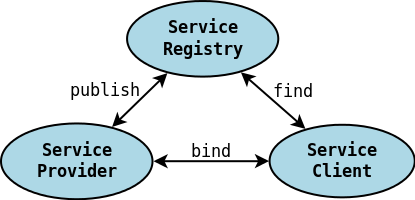
\includegraphics[width=0.6\textwidth]{figuras/soa.png}
   \caption{Arquitetura Orientada a Servi\c{c}os}
\end{figure}

%\section{REST}

\section{Webservices}

Um servi\c{c}o web \'e um sistema de software projetado para suportar interoperabilidade em intera\c{c}\~oes m\'aquina-a-m\'aquina na rede. Possui uma interface descritiva das funcionalidades num formato padronizado (especificamente WSDL). Esta nota\c{c}\~ao abstrata que deve ser implementada por um agente.\cite{w3c-web-04}. 

O agente \'e algo concreto, pode ser um peda\c{c}o de hardware ou software que recebe e envia mensagens. Um exemplo \'e implementar o mesmo servi\c{c}o web, utilizando agentes em diferentes linguagens. Embora o agente seja diferente, o servi\c{c}o Web continua o mesmo.

Servi\c{c}os Web prov\^eem um padr\~ao para a interoperabilidade entre diferentes aplica\c{c}\~oes de software, que executam em diferentes plataformas de software e hardware.

\subsection{RESTful}

RESTFul \'e uma maneira de aplicar os princ\'ipios de design REST para servi\c{c}os web. Uma requisic\c{c}\~ao a um webservice RESTful, utiliza a informa\c{c}\~ao do m\'etodo como um verbo HTTP e a informac\c{c}\~ao do escopo ao qual o verbo ser\'a utilizado na URI. Ao contr\'ario um estilo RPC tende a ignorar o m\'etodo HTTP, procurando pelo m\'etodo a ser utilizado e o escopo na pr\'opria URI. \cite{rest}

Para transfe\^encia de dados utiliza-se formatos gen\'ericos que enfatizam simplicidade e usabilidade pela internet, como XML e JSON. Resource Oriented Architecture A \'e uma arquitetura boa para RESTful webservices. \cite{richardson2008restful}

Os Recursos s\~ao usam um identificador \'unico e persistente, as URIs. A URIs possuem estruturas de diret\'orios, uma URI \'e uma \'arvore com ramos subordinados e superordinados conectando os n\'os. As opera\c{c}\~oes suportas s\~ao m\'etodos HTTP expl\'icitos que n\~ao salvam estado das aplica\c{c}\~oes clientes e s\~ao idempotentes, s\~ao eles:
GET: solicita ao webserver a representa\c{c}\~ao de uma informa\c{c}\~ao de um determinado recurso.
POST: criar um recurso no webserver.
PUT: mudar o estado de um recurso do webserver.
DELETE: remover o recurso ou alterar para um estado vazio.

Uma abordagem utilizando HTTP n\~ao \'e t\~ao interessante para uma aplica\c{c}\~ao de RSSF, j\'a que a quantidade de informa\c{c}\~ao a ser transmitida \'e consideravelmente maior. A figura \ref{bytesTransmitted} faz um comparativo entre o n\'umero de bytes transmitidos de diversos servidores web e seus protocolos.

\begin{figure}[H]
    \label{bytesTransmitted}
    \centering
    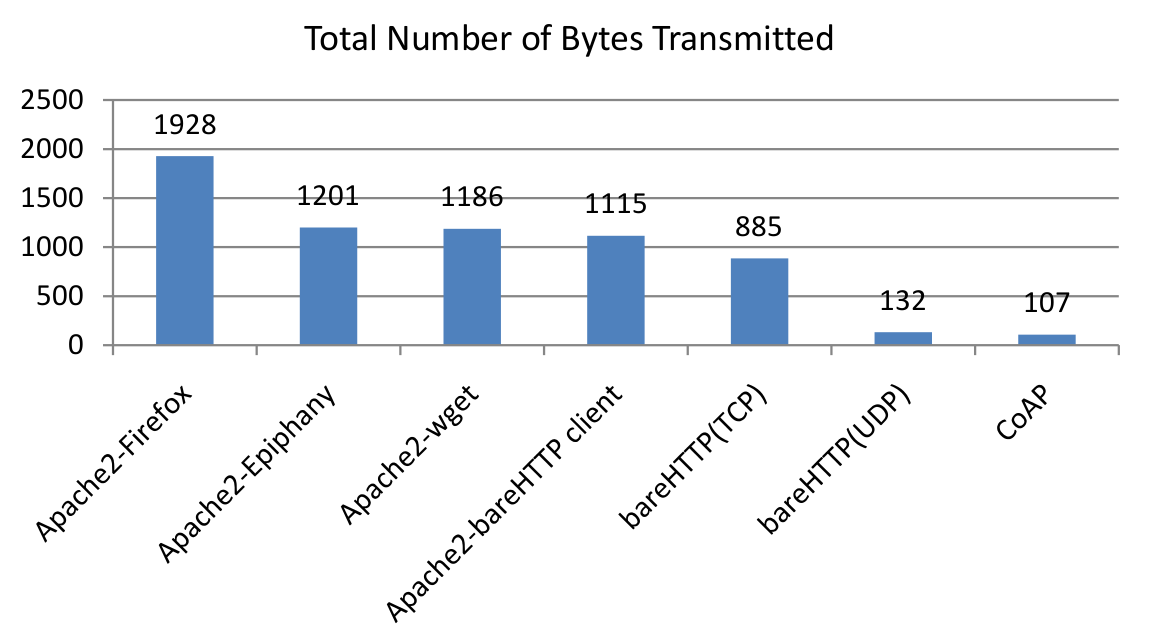
\includegraphics[width=0.9\textwidth]{figuras/bytestransmitted.png}
    \caption{\cite{transportApp}}
\end{figure}

Todos os webservices utilizam o conceito de URI, por\'em de maneiras diferentes. Mas um servi\c{c}o RESTful sempre exp\~oe a URI para cada peda\c{c}o de dado que o cliente quer operar sobre. Os principais competidores aos servi\c{c}os web RESTful s\~ao os RPC-styles.

%\section{Webservices em WSN}

\section{CoAP}

Um dos principais objetivos do CoAP \'e ser uma alternativa protocolo web gen\'erico para redes com dispositivos com restri\c{c}\~ao de energia e mem\'oria.

As vantagens de utilizar um protocolo compat\'ivel com o HTTP s\~ao: a facilidade de integra\c{c}\~ao e o reuso de aplica\c{c}\~oes. CoAP \'e um conjunto REST otimizado para M2M, com suporte a descoberta de recursos, multicast e troca de mensagens ass\'incronas com simplicidade e baixo overhead.

A IETF estabelece as condi\c{c}\~oes m\'inimas para o desenvolvimento de um protocolo de aplica\c{c}\~ao compat\'ivel com HTTP, mas focado em aplica\c{c}\~oes aonde energia e mem\'oria s\~ao escassas. O protocolo CoAP foi projetado levando em considera\c{c}\~ao as restri\c{c}\~oes energ\'eticas e altas taxas de falha na transmiss\~ao dos pacotes em RSSF.

A comunica\c{c}\~ao entre os pontos no CoAP \'e de forma ass\'incrona usando o UDP. A confiabilidade \'e um par\^ametro opcional e funciona atrav\'es de um mecanismo de retransmiss\~ao exponencial.

Possui 4 tipos de mensagem: Confirm\'avel, N\~ao-Confirm\'avel, Confirma\c{c}\~ao (ACK) e Reset. A figura \ref{coapFormat} mostra o formato do pacote.

\subsection{Formato das mensagens}
Uma mensagem CoAP deve caber num \'unico pacote IP, para que seja transmitida numa camada de enlace limitada.
\begin{figure}[H]
    \label{coapFormat}
    \centering
    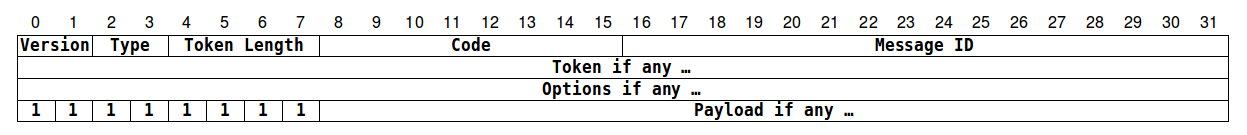
\includegraphics[width=0.6\textwidth]{figuras/formato.png}
    \caption{formato do pacote CoAP  em bits. \cite{draft-ietf-core-coap-18}}
\end{figure}


Os campos do pacote CoAP s\~ao: a vers\~ao do CoAP, implementa\c{c}\~oes devem utilizar este campo com o valor 1. O tipo: campo para definir o tipo da mensagem: Confirm\'avel (0), N\~ao-Confirm\'avel (1) , de Confirma\c{c}\~ao (2) ou Reset (3).

O tamanho do Token: utilizado para controle de requisi\c{c}\~oes e repostas. O tamanho do Token pode variar entre 0 e 8 bytes. Tamanhos entre 9 a 15 s\~ao reservados e n\~ao devem ser usados. \'E um campo sempre gerado pelo cliente CoAP.

O C\'odigo: separados em 3-bit mais significativos para classes e 5-bits menos significativos para detalhe. As classes podem indicar uma requisi\c{c}\~ao (0), uma resposta de sucesso (2), e uma resposta de erro do cliente (4), ou uma resposta de erro do servidor (5), as outras classes s\~ao reservadas. Em um caso especial o c\'odigo 0.00 indica uma mensagem vazia.

O ID da mensagem: usada para deduplica\c{c}\~ao de mensagens e confirma\c{c}\~ao ou reset de mensagens. \'E gerado por quem envia a mensagem, no caso de uma mensagem confirm\'avel ou reset, a resposta deve possuir o ID da mensagem enviada. A implemeta\c{c}\~ao da gera\c{c}\~ao dos IDs est\'a aberta, depende da aplica\c{c}\~ao que o CoAP ser\'a usado, por\'em \'e recomendado que o valor inicial seja rand\^omico.
   
%Codifica\c{c}\~ao das op\c{c}\~oes
\subsection{Transmiss\~ao de Mensagens}
A transmiss\~ao de mensagems \'e controlada basicamente pelos par\^ametros: ACK TIMEOUT, ACK RANDOM FACTOR, MAX RETRANSMIT, NSTART, Leisure e PROBING RATE.

Estes par\^ametros s\~ao respectivamente: o tempo que uma mensagem confirm\'avel aguarda o ACK; fator de randomicidade para gerar os ACK TIMEOUTs subsequentes; contador para o n\'umero m\'aximo de tentativas de retransmiss\~ao; n\'umero limite de intera\c{c}\~oes simult\^aneas mantidas por um servidor.

A Leisure \'e o tempo que o servidor aguarda para responder uma requisi\c{c}\~ao multicast, \'e calculada: $Leisure = S * G / R$. Aonde S \'e o tamanho estimado da reposta, G \'e uma estimativa do tamanho do grupo e R \'e a taxa de transmiss\~ao. PROBING RATE: \'e a taxa m\'edia para transmiss\~ao de dados.

    Estes par\^ametros definem a temporiza\c{c}\~ao do sistema. Os valores padr\~oes s\~ao mostrados na Tabela \ref{coapDefault}.
\begin{table}[h]
\label{coapDefault}
\centering
\begin{tabular}{@{}lllll@{}}
\toprule
Nome & Valor padr\~ao & \\ \midrule
ACK timeout & 2 segundos & \\
ACK random factor & 1.5 & \\
NStart & 1 & \\
Default Leisure & 5 segundos & \\
Probing rate & 1 Byte/segundo & \\
Max retransmit & 4 &  \\ \midrule
\end{tabular}
\caption{Valores padr\~ao do CoAP.}
\end{table}

A retransmiss\~ao \'e controlada por um timeout e um contador. Quando este timeout \'e atigido e o contador \'e menor que valor m\'aximo de retransmiss\~ao a mensagem \'e transmitida, o contador incrementado e timeout duplicado. O modelo de retransmiss\~ao usa um contador de timeouts e uma fun\c{c}\~ao que varia de acordo com o n\'umero de tentativas.

Uma falha na transmiss\~ao ocorre quando atingir o n\'umero m\'aximo de tentavivas ou receber uma mensagem de RESET. Quando receber um ACK a transmiss\~ao da mensagem confirm\'avel \'e completa. O servidor ir\'a ignorar mensagens que chegam por multicast quando n\~ao puder responder nada de \'util.

Na situa\c{c}\~ao aonde possuir uma informa\c{c}\~ao suficientemente nova pode responder na pr\'opria mensagem de confirma\c{c}\~ao (ACK). Essa t\'ecnica \'e chamada de ''Piggy-backed'' um mecanismo de transmiss\~ao para mensagens confirmadas, o cen\'ario \'e ilustrado na Figura \ref{piggyBacked}.\cite{draft-ietf-core-coap-18}
\begin{figure}[H]
   \label{piggyBacked}
   \centering
   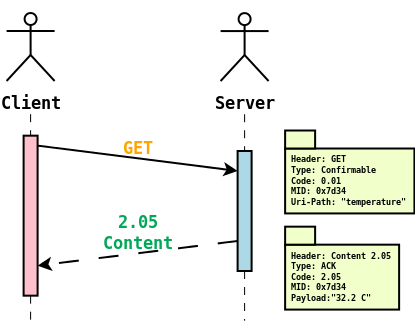
\includegraphics[width=0.6\textwidth]{figuras/piggybacked.png}
   \caption{Resposta na mensagem de confirma\c{c}\~ao, chamado de piggy-backed.}
\end{figure}

\subsection{Requisi\c{c}\~ao e Resposta}

Uma requisi\c{c}\~ao \'e inicializada ao preencher o campo c\'odigo no cabe\c{c}alho do CoAP e gerado um token.
Para finalizar o fluxo \'e necess\'ario que a resposta chegue e o token tem que bater.


Fluxo esperado de requisi\c{c}\~ao sem confirma\c{c}\~ao na figura \ref{nonConfirmable}.
\begin{figure}[H]
   \label{nonConfirmable}
   \centering
   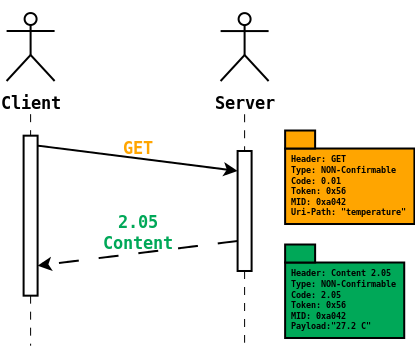
\includegraphics[width=0.6\textwidth]{figuras/nonconfirmable.png}
   \caption{Fluxo esperado de requisi\c{c}\~ao e resposta sem confirma\c{c}\~ao}
\end{figure}

A RFC tamb\'em prev\^e fluxo de requisi\c{c}\~ao com confirma\c{c}\~ao, e resposta separada com confirma\c{c}\~ao. A figura \ref{separateResponse} exemplifica:

\begin{figure}[H]
   \label{separateResponse}
   \centering
   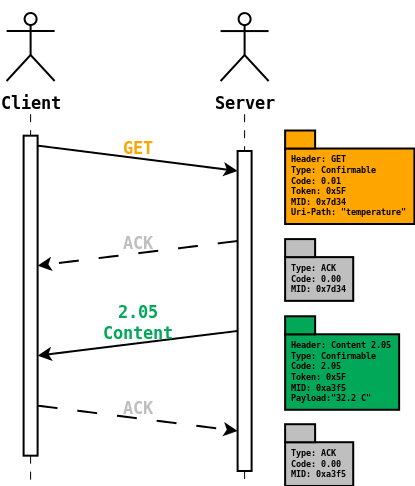
\includegraphics[width=0.6\textwidth]{figuras/separateresponse.png}
   \caption{Fluxo esperado de requisi\c{c}\~ao e resposta com confirma\c{c}\~ao, com resposta separada}
\end{figure}

\subsection{Op\c{c}\~oes}

O CoAP possui diversas op\c{c}\~oes que s\~ao codificadas conforme a tabela abaixo.
As op\c{c}\~oes s\~ao separadas entre eletivas, obrigat\'orias e ....

URI, path, query
observer
\afazer{falta coisa....}


\subsection{Recursos}

A descoberta de recursos \'e feita quando um servidor recebe uma requisi\c{c}\~ao GET para o recurso ~/well-know/core. O servidor CoAP deve responder no formato CORE link Format.\cite{rfc6690} E a descoberta de servi\c{c}os no protocolo CoAP \'e feita atrav\'es de socket Multicast. Os recursos s\~ao identificados por uma URI, e os m\'etodos s\~ao implementados de forma similar ao HTTP.  
\section{EPOS}
O EPOS \'e um sistema operacional multithread com suporte a preemp\c{c}\~ao, foi desenvolvido em C++ que faz uso intenso de programa\c{c}\~ao orientada a aspectos utilizando templates.

Foi projetado utilizando ADESD, Application Driven Embedded System Design, um m\'etodo para projeto de sistemas embarcados orientados \`a aplica\c{c}\~ao. Esta metodologia guia o desenvolvimento paralelo de hardware e software al\'em de manter portabilidade. O EPOS possui porte para as seguintes arquiteturas: MIPS, IA32, PowerPC, H8, Sparc, AVR e ARM. \cite{eposProject}

Possui abstra\c{c}\~oes para entidades temporais como rel\'ogio, alarme e cron\^ometro, biblioteca com estruturas de dados e sequenciadores. Permitindo o uso de ferramentas para gera\c{c}\~ao automatizada de abstra\c{c}\~oes de sistemas. A portabilidade \'e atingida utilizando entidades chamados de Mediadores de Hardware que fornecem interfaces simples para acesso as fun\c{c}\~oes espec\'ificas de arquitetura. Estas interfaces s\~ao utilizadas por entidades abstratas como alarmes e threads peri\'odicas. Abaixo uma a figura \ref{eposOverview} ilustrando a vis\~ao geral do EPOS.

\begin{figure}[H]
   \label{eposOverview}
   \centering
   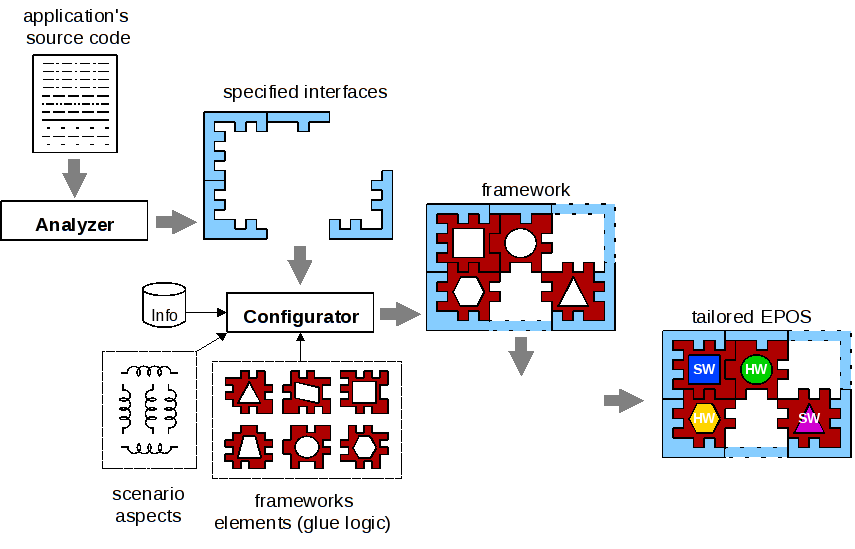
\includegraphics[width=0.8\textwidth]{figuras/eposOverview.png}
   \caption{Overview do EPOS.}
\end{figure}

 
O EPOS tamb\'em possui uma interface de software/hardware que abstrai de sensores de forma uniforme, definindo classes de dispositivos baseados numa finalidade.\cite{epos}
%Inserir figura da arquitetura do EPOS.

A infraestrutura de comunicaca\c{c}\~ao do EPOS para redes de sensores sem-fio \'e implementada pelo protocolo C-MAC, Configurable MAC, que prov\^e suporte a comunicaca\c{c}\~ao de baixo n\'ivel (MAC - Medium Access Control)

\section{Trabalhos Relacionados}

\subsection{OpenWSN}

O projeto OpenWSN \'e um projeto de redes de sensores sem fio de c\'odigo aberto e confia na comunidade para manter atualizado e encontrar erros. Possui uma implementa\c{c}\~ao completa de c\'odigo aberto, das pilhas de protocolos padr\~oes pra Internet das Coisas.

E com a primeira implementa\c{c}\~ao aberta do padr\~ao 802.15.4e, Time Synchronized Channel Hopping.

Por serem sincronizados os motes precisam acordar apenas para transmitir ou receber e periodicamente se comunicar para manter a rede sincronizada quando estiver inativo. Este overhead de temporiza\c{c}\~ao \'e pequeno, cerca de 0.02\% de ciclo de trabalho do r\'adio. \cite{openWSNPaper}

O pilha de protocolos \'e totalmente em C e pode ser compilada em qualquer toolchain que suporte uma plataforma alvo. OpenWSN j\'a foi portado para as seguintes arquiteturas: ARM, AVR, ...

Possui porte para diversas plataformas de microcontroladores de 16 bits e para as arquiteturas mais novas de 32 bits dos cortex-M. O projeto possui diversas ferramentas para depura\c{c}\~ao, simula\c{c}\~ao e ambiente necess\'ario para integrar as aplica\c{c}\~oes a Internet.\cite{openWSN}

Resultados experimentais de uma rede de motes demonstram que os r\'adios operam num ciclo m\'edio de trabalho de $0.1\%$ e uma m\'edia de 0.68 microA em hardware comum. Este consumo baixo permite uma vasta gama de aplica\c{c}\~oes.

Para utilizar \'e necess\'ario baixar os seguintes reposit\'orios:
\begin{description}
    \item [Software de sistema:] https://github.com/openwsn-berkeley/openwsn-fw
    \item [Ferramentas para desenvolvimento:] https://github.com/openwsn-berkeley/openwsn-sw 
    \item[Implementa\c{c}\~ao do CoAP:] https://github.com/openwsn-berkeley/coap
\end{description}


\subsection{Contiki}
O Contiki \'e um sistema operacional criado por Adam Dunkels em 2000, escrito em C, de c\'odigo aberto para sistemas com restri\c{c}\~ao de recursos comunicam-se numa rede. Foi desenvolvido para ser um sistema operacional para Internet das coisas. Possui uma camada de abstra\c{c}\~ao RESTful para web services chamada Erbium, que implementa o protocolo CoAP.

Cada processo no Contiki possui bloco de controle, que cont\'em informa\-\c{c}\~oes de tempo de execu\c{c}\~ao do processo e uma refer\^encia para uma protothread, na qual o c\'ogido \'e armazenado na ROM. 

Programas escritos num modelo dirigido a eventos, geralmente s\~ao implementados como m\'aquinas de estados expl\'icitas, que com um grande n\'umero de estados o c\'odigo come\c{c}a a se tornar complexo, dif\'icil de entender e depurar. Estas foram as principais motiva\c{c}\~oes para que fosse desenvolvido um modelo de programa\c{c}\~ao diferente, utilizado nos projetos desenvolvidos por Adam, a pilha uIP e do Contiki.\cite{Dunkels05protothreads}

O conceito protothread foi desenvolvido por Adam Dunkels em 2005, uma combina\c{c}\~ao entre eventos e threads, possuem comportamentos de bloqueio e espera, que permite o intersequenciamento dos eventos, gerando um baixo overhead de mem\'oria por n\~ao necessitar de salvamento de contexto.

As limita\c{c}\~oes dessa t\'ecnicas s\~ao: vari\'aveis autom\'aticas n\~ao s\~ao preservadas Stack durante trocas de contexto entre as protothreads. Elas podem ser utilizadas durante uma protothread mas devem ser salvas antes da execu\c{c}\~ao de do m\'etodo WAITING. Al\'em disso programas que utilizam protothreads n\~ao podem utilizar switch case, caso o fizer um erro de compila\c{c}\~ao \'e esperado.

Cada protothread consome 2 bytes de mem\'oria, que s\~ao utilizados para armazenar a continuidade local, uma referencia utilizada em um pulo condicional durante a execu\c{c}\~ao da thread. \'E um m\'etodo similar ao mecanismo de Duffy e Co-rotina em C. \cite{duffyMechanism}

O Contiki prop\~oe uma estrat\'egia de ciclos de trabalho que consegue manter um n\'o comunic\'avel em uma rede, por\'em com seus r\'adios desligados em aproximadamente 99\% do tempo.\cite{Dunkels11thecontikimac}

\subsection{LibCoap}
LibCoap \'e uma biblioteca implementada em C do protocolo CoAP. Possui 292K de tamanho compilada estaticamente em sua vers\~ao 4.0.1.
A licensa da biblioteca \'e GPL (2 ou maior) ou licensa BSD revisada.

Possui uma su\'ite de testes para regress\~ao, utilizando o framework de testes CUnit (http://cunit.sourceforge.net/). A documenta\c{c}\~ao pode ser encontrada em: http://libcoap.sourceforge.net/.

\'E uma biblioteca auto-condida, que possui parser do protocolo e fun\c{c}\~oes b\'asicas de rede. Depende de implementa\c{c}\~ao de sockets tipo BSD e malloc. Possui implementa\c{c}\~ao de Hash, String e URI utilizados para montar os pacotes CoAP.

Possui um m\'odulo de rede, aonde \'e implementado as fun\c{c}\~oes de envio/recebimento de requisi\c{c}\~oes e respostas, com confirma\c{c}\~ao, sem confirma\c{c}\~ao, mensagem de reset e erros.

\'E poss\'ivel selecionar a camada de transporte \'e necess\'ario selecionar utilizando flags de preprocessamento. O padr\~ao \'e socket POSIX. A pilha uIP \'e selecionada com a flag -DWITH\textunderscore CONTIKI, ou para selecionar a pilha lwIP -DWITH\textunderscore LWIP.

\subsection{CantCoap}
\'E uma implementa\c{c}\~ao em C++ desenvolvida por Ashley Mills em 2013. Utiliza uma licensa similar a.

Esta biblioteca foca na simplicidade e oferece uma conjuto m\'inimo para montar pacotes CoAP.
Tamb\'em \'e poss\'ivel montar os pacotes CoAP a partir de uma sequ\^encia de caracteres recebidos de uma placa de rede. Abaixo exemplos de uso da biblioteca retirados de https://github.com/staropram/cantcoap.

\lstdefinestyle{customc}{
  belowcaptionskip=1\baselineskip,
  breaklines=true,
  xleftmargin=\parindent,
  language=C++,
  showstringspaces=false,
  basicstyle=\scriptsize\ttfamily,
  keywordstyle=\bfseries\color{black},
  commentstyle=\itshape\color{blue},
  identifierstyle=\color{black},
  stringstyle=\color{red},
}

\lstset{escapechar=@,style=customc}

Abaixo um exemplo de uso para montar um pacote e enviar:

\begin{lstlisting}
CoapPDU *pdu = new CoapPDU();
pdu->setType(CoapPDU::COAP_CONFIRMABLE);
pdu->setCode(CoapPDU::COAP_GET);
pdu->setToken((uint8_t*)"\3\2\1\0",4);
pdu->setMessageID(0x0005);
pdu->setURI((char*)"test",4);

/* send packet */
ret = send(sockfd,pdu->getPDUPointer(),pdu->getPDULength(),0);
\end{lstlisting}

Quando receber a mensagem a forma de uso \'e mostrada abaixo:
\begin{lstlisting}
// receive packet
ret = recvfrom(sockfd,&buffer,BUF_LEN,0,recvAddr,recvAddrLen);
CoapPDU *recvPDU = new CoapPDU((uint8_t*)buffer,ret);
if(recvPDU->validate()) {
    recvPDU->getURI(uriBuffer,URI_BUF_LEN,&recvURILen);
    ...
}
\end{lstlisting}

Por ser uma biblioteca bem simplificada e n\~ao possuir depend\^encias diretas com a implementa\c{c}\~ao da camada de transporte e ser c\'odigo livre, foi escolhida para a implementa\c{c}\~ao teste do trabalho.


%\chapter{Proposta}
%Este trabalho prop\~oes a implementa\c{c}\~ao de uma biblioteca que utiliza a camada UDP do EPOS para dar suporte ao protocolo CoAP.

O trabalho tamb\'em consiste na implementa\c{c}\~ao de uma aplica\c{c}\~ao para gateway GPRS/Zigbee utilizando o EPOS e um componente de hardware que ser\'a acoplado ao EposMoteII. Este componente esta sendo desenvolvido em paralelo por um colega de laborat\'orio.

O desenvolvimento da aplica\c{c}\~ao no EPOS que ser\'a respons\'avel pelo roteamento de mensagens para Internet utiliza a tecnologia GPRS, provida por um m\'odulo GSM/GPRS da Quectel o M95.

As principais fun\c{c}\~oes deste gateway s\~ao receber os dados da rede de sensores e encaminh\'a-las para um servidor remoto que armazenar\'a essas informa\c{c}\~oes e exibir\'a de forma conveniente para o usu\'ario final.

As fun\c{c}\~oes a serem desenvolvidas na aplica\c{c}\~ao do gateway s\~ao:

\begin{itemize}[noitemsep,topsep=0pt,parsep=0pt,partopsep=0pt]
    \item Configura\c{c}\~ao SMS
    \item Envia mensagem SMS
    \item Recebe mensagem SMS
    \item Configura\c{c}\~ao contexto PDP
    \item Configura\c{c}\~ao GPRS
    \item Configura\c{c}\~ao TCP/IP
    \item Manter uma conex\~ao TCP/IP 
\end{itemize}

\section{Metas}
Entregar um m\'odulo simplificado do procotolo CoAP no primeiro semestre e testar as funcionalidades no modem GSM/GPRS.
Desenvolver a aplica\c{c}\~ao no EPOS no segundo semestre e fazer testes de integra\c{c}\~ao.

\section{Cronograma}
\begin{ganttchart}[
    vgrid, hgrid
    ] {1}{21}
    \gantttitle {Trabalho de Conclus\~ao de Curso}{21} \\
    \gantttitlelist {3,...,12}{2}\\
    \ganttgroup {2013.1} {1}{10}\\
    \ganttbar {Estudar EPOS} {1}{4}\\
    \ganttbar {Estudar EPOSMoteII}{1}{4}\\
    \ganttbar {Estudar modem GPRS}{1}{4}\\
    \ganttbar {Levantar requisitos libcoap no EPOS} {3}{4} \\
    \ganttbar {Levantar requisitos do HW} {1}{6}\\
    \ganttbar {Implementa\c{c}\~ao do CoAP} {3}{10} \\
    \ganttbar {Testar modem GPRS} {4}{10} \\
    \ganttbar {Desenvolvimento do prot\'otipo do HW} {7}{10}\\
    \ganttmilestone {Relat\'orio de TCC I}{10}\\
    \ganttnewline[thick, blue]
    \ganttgroup {2013.2}{11}{20} \\
    \ganttbar {Implementa\c{c}\~ao do Gateway} {11}{18}\\
    \ganttbar {Testes de Integra\c{c}\~ao} {19}{20}\\
    \ganttbar {Documenta\c{c}\~ao do trabalho} {1}{20} \\
    \ganttmilestone {Relat\'orio de TCC II}{20}

    \ganttlink {elem2}{elem7}
    \ganttlink {elem3}{elem7}
    \ganttlink {elem5}{elem7}
    \ganttlink {elem1}{elem11}
    \ganttlink {elem4}{elem11}
    \ganttlink {elem7}{elem10}
    \ganttlink {elem11}{elem12}
    \ganttlink {elem12}{elem11}
    \ganttlink {elem11}{elem13}
    \ganttlink {elem10}{elem13}

\end{ganttchart}

\section{Resultados parciais}

Abaixo est\~ao listadas as atividades conclu\'idas at\'e o momento:
\begin{itemize}
    \item Estudar EPOS.
    \item Estudar EPOSMoteII.
    \item Estudar modem GPRS.
    \item Levantar requisitos libcoap no EPOS.
    \item Levantar requisitos do HW.
    \item Implementa\c{c}\~ao do CoAP: a parte de valida\c{c}\~ao de um pacote CoAP foi feita com TDD e est\'a dispon\'ivel no site: (TODO).
    \begin{itemize}[noitemsep,topsep=0pt,parsep=0pt,partopsep=0pt]
        \item Ao receber uma mensagem de confirma\c{c}\~ao, remove da lista a mensagem que n\~ao havia sido confirmada utilizando o id.
        \item Ao receber uma mensagem confirm\'avel, envia uma mensagem de confirma\c{c}\~ao.
        \item Repassar mensagem para controle de Requisi\c{c}\~ao e Reposta.
        \item Adicionar a lista de mensagem recebidas.
        \item Enviar mensagem n\~ao confirm\'avel.
        \item Enviar mensagem confirm\'avel e adicionar na lista de confirma\c{c}\~oes pendentes.
        \item Reenviar a mensagem que est\'a na lista de confirma\c{c}\~ao pendente e reconfigurar o pr\'oximo reenvio.
    \end{itemize}
    
    \item Testes no m\'ouldo GPRS:
        \begin{itemize}[noitemsep,topsep=0pt,parsep=0pt,partopsep=0pt]
            \item Enviar Mensagem
            \item Receber Mensagem
            \item Criar socket TCP
            \item Enviar mensagem via socket
            \item Receber mensagem via socket
            \item Fazer requisi\c{c}\~ao HTTP para um webserver, foi poss\'ivel utilizando os comandos propriet\'arios do modem.
        \end{itemize}
    \item Desenvolvimento do prot\'otipo do HW.
\end{itemize}

\subsection{Atividades pendentes}
As atividades que ser\~ao feitas ao longo do segundo semestre:
\begin{itemize}
    \item Implementa\c{c}\~ao do Gateway.
    \item Testes de Integra\c{c}\~ao.
    \item Documenta\c{c}\~ao do trabalho.
    \item Relat\'orio de TCC II.
\end{itemize}


\chapter{Desenvolvimento}
Este trabalho implementa uma biblioteca que utiliza a camada UDP do EPOS para dar suporte ao protocolo CoAP, uma aplica\c{c}\~ao gateway GPRS/802.14.5 utilizando o EPOS e um componente de hardware GPRS que ser\'a acoplado ao EposMoteII.

Para isto foram realizados diversos estudos durante o desenvolvimento do protocolo, pesquisas para escolher um m\'odulo GPRS adequado a tarefa. Al\'em disso testes de valida\c{c}\~ao dos sistemas de software e valida\c{c}\~ao do m\'odulo GPRS, levantamento de requisitos para porte de uma biblioteca CoAP para o EPOS (libCoap, libCantCoap, microCoap, entre outras) e EPOSMoteII.

Porte da biblioteca para o EPOS. Utilizando testes para validar o funcionamento entre diferentes arquiteturas e compiladores. A execu\c{c}\~ao dos testes foi feita no Qemu.

Implementa\c{c}\~ao dos mecanismos de transmiss\~ao para mensagens confirm\'aveis e n\~ao-confim\'aveis, requisi\c{c}\~ao e resposta.

A aplica\c{c}\~ao que ser\'a respons\'avel pelo roteamento de mensagens para Internet utiliza a tecnologia GPRS, provida por um m\'odulo GSM/GPRS da Quectel o M95.

\section{Levantamento de Requisitos}
Infraestrutura flex\'ivel para a contru\c{c}\~ao de aplica\c{c}\~oes embarcadas em modelo de webservices utilizando redes de sensores sem fio.

O usu\'ario ir\'a acessar a rede de sensores sem fio por uma aplica\c{c}\~ao html5, hospedada em http://minhascoisas.io.
Nesta aplica\c{c}\~ao \'e poss\'ivel enviar requisi\c{c}\~oes para a rede de sensores de teste e listar os servi\c{c}os oferecidos.

\subsection{Requisitos Funcionais}
Coletar informa\c{c}\~ao do ambiente atrav\'es de sensores e transmit\'i-las atrav\'es da Internet. F\'acil integra\c{c}\~ao com a Internet mesmo em locais sem rede WIFI.

As principais fun\c{c}\~oes deste gateway s\~ao receber os dados da rede de sensores e encaminh\'a-las para um servidor remoto que armazenar\'a essas informa\c{c}\~oes e exibir\'a de forma conveniente para o usu\'ario final.

Ser\'a poss\'ivel comunicar-se em tempo real com a rede de sensores, utilizando um m\'odulo GPRS que ir\'a repassar as requisi\c{c}\~oes e respostas alimentadas pelo usu\'ario.

As fun\c{c}\~oes a da aplica\c{c}\~ao do gateway s\~ao:
\begin{enumerate}
    \item Configura\c{c}\~ao, envio e recebimento de SMS;
    \item Configura\c{c}\~ao contexto PDP, Configura\c{c}\~ao GPRS;
    \item Configura\c{c}\~ao TCP/IP e manuten\c{c}\~ao de conex\~ao TCP/IP.
\end{enumerate}

\subsection{Requisitos N\~ao Funcionais}

Os webservices que v\~ao executar nos motes devem herdar a caracteristica de baixo consumo energ\'etico para que possam durar por anos, e serem extens\'iveis, podendo ser reutilizada em outras arquiteturas.

Al\'em os servi\c{c}os ser\~ao listatos utilizando o padr\~ao \cite{rfc6690} disso os dados captados por sensores ser\~ao disponibilizados na forma de webservices CoAP, protocolo espec\'ifico para este tipo de aplicac\c{c}\~ao.

A padroniza\c{c}\~ao na comunica\c{c}\~ao visa facilitar a interconex\~ao dos sistemas de diversas plataformas.

Caracter\'isticas destes sistemas s\~ao eficiente em:
    \begin{itemize}
        \item Armazenamento: deve ser suficientemente pequeno para ser utilizado em microcontroladores.
        \item Energia: cosumir pouca energia para longa durabilidade com bateria.
        \item Valor: utilizar uma infraestrutura de hardware simples para realizar as tarefas.
    \end{itemize}


\section{Especifica\c{c}\~ao}
\subsection{Arquitetura}

A figura \ref{arquitetura} ilustra a interconex\~ao entre os nodos da rede.

\begin{figure}[h]
   \label{arquitetura}
   \centering
   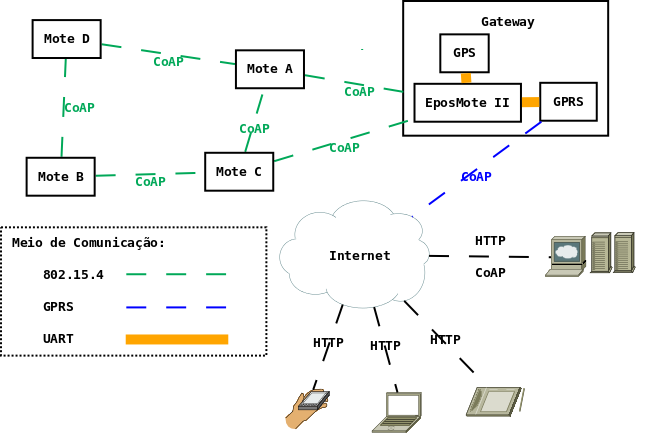
\includegraphics[width=0.8\textwidth]{figuras/arquitetura.png}
   \caption{Vis\~ao geral sobre comunica\c{c}\~ao do sistema.}
\end{figure}

\subsection{Componentes}
O CoAP implementado \'e composto pelos seguintes componentes:



A implementa\c{c}\~ao consiste num m\'odulo que trata requisi\c{c}\~oes, encapsula em pacotes e transmite por mecanimos de transmiss\~ao baseados em \cite{draft-ietf-core-coap-18}.

A biblioteca utilizada para montar o pacote CoAP foi:\\https://github.com/staropram/cantcoap.git. Na qual enviei algumas corre\c{c}\~oes e testes para facilitar a verifica\c{c}\~ao da execu\c{c}\~ao correta dos algoritmos internos durante mudan\c{c}as no c\'odigo. As altera\c{c}\~oes podem ser visualisadas aqui:\\https://github.com/staropram/cantcoap/commits?author=rafaeldelucena.

Para o funcionamento desta biblioteca no EPOS, e para utilizar uma MTU limitada a 128 bytes utilizo um buffer com um valor m\'aximo e armazeno os dados do pacote no buffer. Foi necess\'ario alterar os tipos das vari\'aveis para se adquerem ao EPOS.

O desenvolvimento de um mecanismo de retransmiss\~ao de mensagens n\~ao-confirmadas utilizando uma lista ordenada. Mecanismo de requisic\c{c}\~o e resposta, as requisi\c{c}\~oes pendentes foram armezenadas num Hash com a chave sendo o token gerado pelo cliente.

O protocolo CoAP foi modelado conforme \'e mostrado na figura \ref{uml} abaixo:
\begin{figure}[h]
   \label{uml}
   \centering
   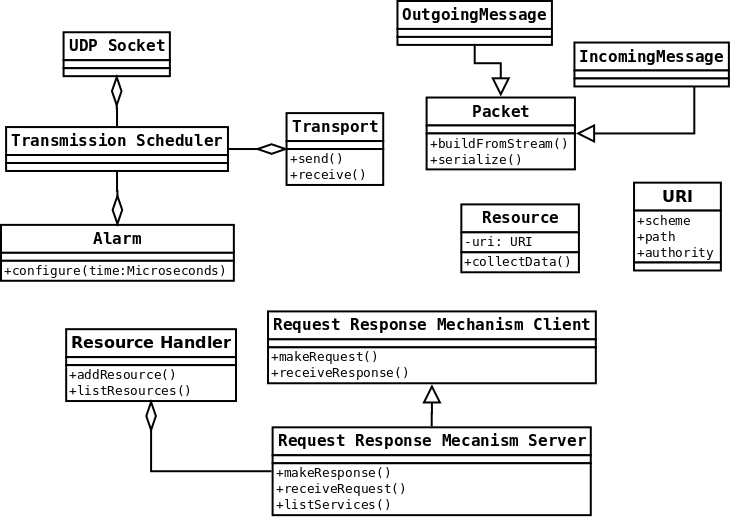
\includegraphics[width=0.9\textwidth]{figuras/uml.png}
   \caption{Diagrama UML das entidades de software implementadas.}
\end{figure}


\begin{figure}[h]
   \label{uml}
   \centering
   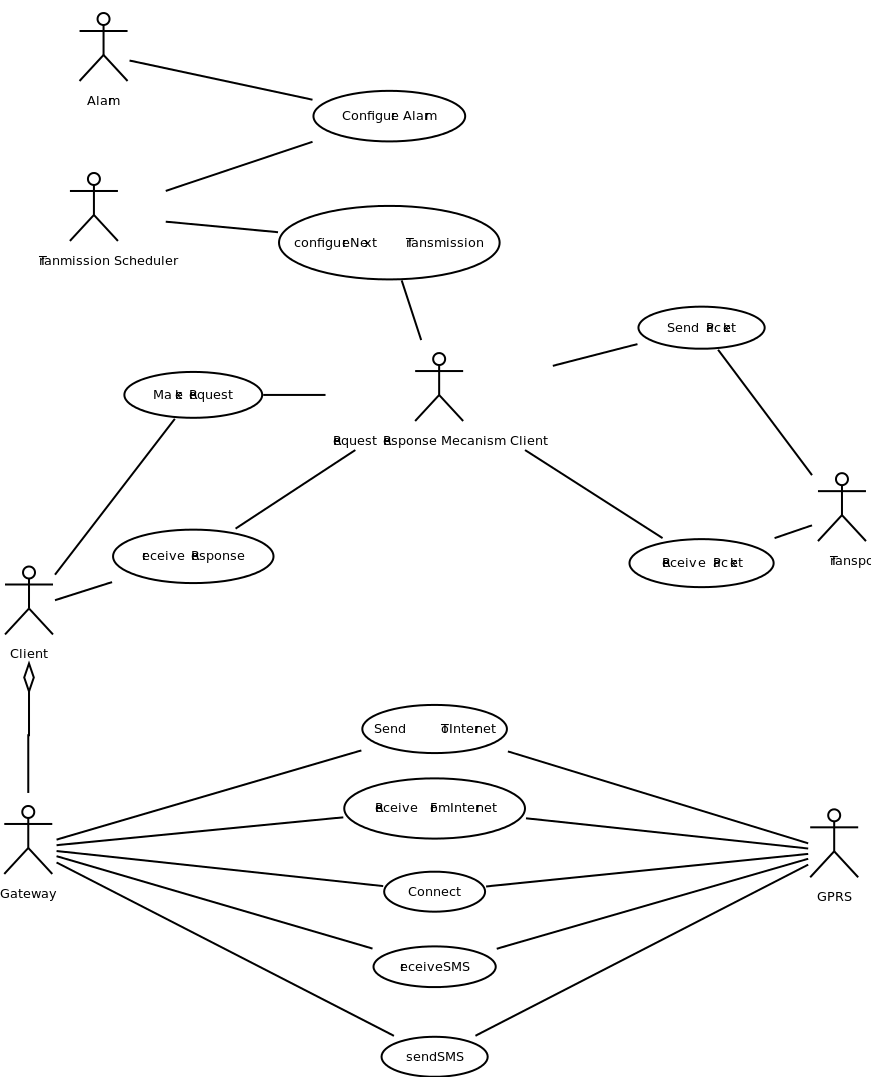
\includegraphics[width=0.8\textwidth]{figuras/casodeuso.png}
   \caption{Diagrama de casos de uso.}
\end{figure}

Para validar o comportamento utilizei alguns testes da pr\'opria biblioteca CoAP portados para o EPOS. Foi necess\'ario implementar a fun\c{c}\~ao assert. J\'a que seria bem mais trabalhoso adicionar uma ferramenta de testes no sistema de build do EPOS.

\section{Testes}
Testes do cliente:
Fazendo uma requisi\c{c}\~ao confirm\'aveis e n\~ao-confirm\'aveis do tipo: GET, POST, PUT, DELETE.
Recebendo respostas: válidas e inválidas.


Testes do Servidor:
Recebendo e respondendo requisi\c{c}\~oes: que possui recurso, que n\~ao possui, descoberta de recurso.

\subsection{Testes na placa de desenvolvimento do m\'ouldo GPRS}
Os testes feitos foram: Enviar e recebimento de mensagens; criar socket TCP, enviar e receber mensagem via socket, fazer requisi\c{c}\~ao HTTP, foi poss\'ivel utilizando os comandos propriet\'arios do modem.


\chapter{Avalia\c{c}\~ao}
\section{An\'alise Funcional}
\subsection{Limita\c{c}\~oes Funcionais}
A falta de uma implementaca\c{c}\~ao segura, utilizando os padr\~oes DTLS.
\section{An\'alise Estrutural}
\section{An\'alise de Desempenho}
O tempo de execu\c{c}\~ao das principais fun\c{c}\~oes foi medido. Abaixo a tabela \ref{comparacaoCoap}, que faz um comparativo com as diversas arquituras e opera\c{c}\~oes entres as principais solu\c{c}\~oes livres.

\begin{table}[h]
\label{comparacaoCoap}
\centering
\begin{tabular}{@{}lllll@{}}
\toprule
OS & CoAP & Size &  Memory &  &  \\ \midrule
EPOS &  CantCoap &  &  &  \\
Contiki &  Erbium &  &  &  \\
Contiki &  libcoap &  &  &  \\
TinyOS &  libcoap &  &  &  \\ \bottomrule
\end{tabular}
\caption{Compara\c{c}\~ao das implementa\c{c}\~oes}
\end{table}

%\lstdefinestyle{customc}{
%  belowcaptionskip=1\baselineskip,
%  breaklines=true,
%  xleftmargin=\parindent,
%  language=C,
%  showstringspaces=false,
%  basicstyle=\footnotesize\ttfamily,
%  keywordstyle=\bfseries\color{green!40!black},
%  commentstyle=\itshape\color{purple!40!black},
%  identifierstyle=\color{blue},
%  stringstyle=\color{orange},
%}
%
%\lstdefinestyle{customasm}{
%  belowcaptionskip=1\baselineskip,
%  frame=L,
%  xleftmargin=\parindent,
%  language=[x86masm]Assembler,
%  basicstyle=\footnotesize\ttfamily,
%  commentstyle=\itshape\color{purple!40!black},
%}
%
%\lstset{escapechar=@,style=customc}
%
%\begin{lstlisting}
%#include <stdio.h>
%#define N 10
%/* Block
% * comment */
% 
%int main()
%{
%    int i;
% 
%    // Line comment.
%    puts("Hello world!");
% 
%    for (i = 0; i < N; i++)
%    {
%        puts("LaTeX is also great for programmers!");
%    }
% 
%    return 0;
%}
%\end{lstlisting}


\chapter{Considera\c{c}\~oes Finais}
O objetivo principal foi atigindo, o desenvolvimento de um gateway simplificado para redes de sensores que utilizem o protocolo CoAP para disponibilizar servi\c{c}os de sensoriamente e atua\c{c}\~ao.

Al\'em disso o consumo de energia e o espa\c{c}os de armazenamento s\~ao muito baixos, respeitando os requis\'itos desse tipo de aplica\c{c}\~ao.

Entres os trabalhos futuros poss\'iveis se destacam os seguintes:
A implementa\c{c}\~ao do protocolo coaps, utilizando DLTS para comunica\c{c}\~ao segura entre os n\'os.

Uma implementa\c{c}\~ao de servidor CoAP completa para executar utilizando a plataforma do EPOSMote II.

Implementa\c{c}\~ao de um gateway que utilize Software Defined Radio, assim apenas um transceiver ser\'a necess\'ario para
fazer a integra\c{c}\~ao com a Internet.

Um gerador de c\'odigo que utiliza como entrada uma linguagem de especifica\c{c}\~ao dos poss\'iveis recursos e como sa\'ida c\'odigo ANSI C m\'inimo de um servidor web utiliza CoAP e seus respectivos recursos. Este gerador deve ser gen\'erico suficiente para ser f\'acil a adapta\c{c}\~ao de diferentes pilhas UDP/IP, arquiteturas e tipos de sensores.


\bibliography{bibliografia}{}
\bibliographystyle{ufscThesis/ufsc-alf}

%--------------------------------------------------------
% Elementos pós-textuais

%\anexo
%\chapter{C\'odigo Desenvolvido}
%\lstdefinestyle{customc}{
  belowcaptionskip=1\baselineskip,
  breaklines=true,
  xleftmargin=\parindent,
  language=C++,
  showstringspaces=false,
  basicstyle=\scriptsize\ttfamily,
  keywordstyle=\bfseries\color{green!40!black},
  commentstyle=\itshape\color{blue},
  identifierstyle=\color{blue!20!black},
  stringstyle=\color{red},
}

\subsection{CoAP}

\begin{lstlisting}

#ifndef __coap_packet_h__
#define __coap_packet_h__

#include <coap_pdu.h>

__BEGIN_SYS

class CoapPacket : public CoapPDU
{
    public:
        static const int ackTimeout = 2000000;
        static const double ackRandomFactor = 1.5;
        static const int maxRetransmit = 4;
        static const int nStart = 1;

        CoapPacket(const UDP_Address & to);
        CoapPacket(const UDP_Address & from, const char * data, unsigned len);
        CoapPacket(CoapPDU * pdu);
        CoapPacket();
        ~CoapPacket();

        bool isConfirmable();
        bool isConfirmed();
        bool isFailure() {return false;};
        void setConfirmed();
        void reset();
        virtual void update() {kout << "Packet update" << endl;};
        UDP_Address remote() const;
        int getToken();
    protected:
        void generateNewToken(unsigned int len);
    private:
        static const int _maxPDUSize = 100;
        bool _isConfirmed;
        UDP_Address _remote;
        u8 _pduBuffer[_maxPDUSize];
        Alarm * _alarm;
};

class CoapACK : public CoapPacket
{
    public:
        CoapACK(int id) : CoapPacket() {
            setType(CoapPacket::COAP_ACKNOWLEDGEMENT);
            setCode(CoapPacket::COAP_EMPTY);
            setMessageID(id);
        }
};

class CoapConfirmable : public CoapPacket {
    public:
        CoapConfirmable(CoapPacket::Code code);
        ~CoapConfirmable();
        void update();
        bool isFailure();
        void reset();
    private:
        Alarm * _alarm;
        int _retransmissionCounter;
        int _timeout;
};

__END_SYS

#endif /*__coap_packet_h__*/


#ifndef __coap_request_h__
#define __coap_request_h__

#include <coap_packet.h>

__BEGIN_SYS

class CoapRequest : public CoapConfirmable
{
    public:
        CoapRequest(CoapPacket::Code code, const char* uri);
        virtual void onSuccess();
        virtual void onError();
        static void incomingResponse(CoapPacket * packet);
        bool wasAnswered() { return (_response != 0);}
    private:
        void addResponse(CoapPacket *);
        void addAsPending();
        static CoapRequest * removePendingByToken(int token);
        static unsigned int indexByToken(int token);
        static const int _maxPDUSize = 100;
        static const int _maxPending = 100;
        char _uriBuffer[_maxPDUSize];
        int _uriSize;
        static CoapRequest * _pendingRequests[_maxPending];
        CoapPacket * _response;
};

__END_SYS

#endif /*__coap_request_h__*/


#ifndef __coap_response_h__
#define __coap_response_h__

__BEGIN_SYS

class CoapPacket;

template <class T>
class CoapResponse : public CoapPacket
{
    public:
        CoapResponse(T data, CoapRequest * r);
        ~CoapResponse();
    private:
        T * _data;
};

__END_SYS

#endif /*__coap_response_h__*/


#ifndef __coap_socket_h_
#define __coap_socket_h_

#include <udp.h>
#include <coap_packet.h>
#include <utility/queue.h>

#define COAP_PORT 5683

__BEGIN_SYS

class CoapSocket : public UDP::Socket
{
public:
    CoapSocket(const UDP_Address & local);
    ~CoapSocket();
    void sendPacket(CoapPacket * pdu);
    void sendPacket(const CoapPacket & pdu);
    void received(const UDP_Address & from, const char* msg, unsigned int len);
};

__END_SYS

#endif /* __coap_socket_h_ */


#include <coap_packet.h> 
#include <coap_socket.h>
#include <utility/handler.h>
__BEGIN_SYS

class CoapTransport
{
    public:
    static Function_Handler * dispatcher();
    static void incoming(CoapPacket * in);
    static void outgoing(CoapPacket * out);
    
    private:
    CoapTransport();
    ~CoapTransport();
    void addNonConfirmed(CoapPacket* p);
    static void dispatch();
    CoapSocket * _socket;
    Queue<CoapPacket> * _queue;
    Function_Handler * _handler;
    static CoapTransport * getInstance();
    static CoapTransport * _instance;
};
__END_SYS


#include <utility/random.h>
#include <utility/string.h>
#include <coap_packet.h>
#include <coap_transport.h>

__BEGIN_SYS

/*
 * For a new Confirmable message, the initial timeout is set
 * to a random duration (often not an integral number of seconds)
 * between ACK_TIMEOUT and (ACK_TIMEOUT * ACK_RANDOM_FACTOR) (see
 * Section 4.8)
 * */
CoapPacket::CoapPacket(const UDP_Address & to) : CoapPDU(_pduBuffer, _maxPDUSize, 4),
     _remote(to)
{
    setVersion(1);
    _isConfirmed = false;
    int range = (CoapPacket::ackTimeout * CoapPacket::ackRandomFactor) - CoapPacket::ackTimeout;
    int rand = Pseudo_Random::random() % range;
    setMessageID(rand);
}

CoapPacket::CoapPacket() : CoapPDU(_pduBuffer, _maxPDUSize, 4), _remote(UDP_Address("10.0.2.15:5863"))
{
    setVersion(1);
    _isConfirmed = false;
    int range = (CoapPacket::ackTimeout * CoapPacket::ackRandomFactor) - CoapPacket::ackTimeout;
    int rand = Pseudo_Random::random() % range;
    setMessageID(rand);
}

CoapPacket::CoapPacket(const UDP_Address & from, const char * data, unsigned len) : CoapPDU(_pduBuffer, _maxPDUSize, len),
    _remote(from)
{
    strncpy((char*)_pduBuffer, data, len);
}

CoapPacket::CoapPacket(CoapPDU * pdu) : CoapPDU(pdu->getPDUPointer(), _maxPDUSize, pdu->getPDULength()),
    _remote(UDP_Address("10.0.2.15:5863"))
{
    setMessageID(pdu->getMessageID());
}

void CoapPacket::reset()
{
    CoapPDU::reset();
    _isConfirmed = false;
}

int CoapPacket::getToken()
{
    return atol((char*)getTokenPointer());
}

CoapPacket::~CoapPacket()
{
}

CoapConfirmable::~CoapConfirmable()
{
    if (_alarm) delete _alarm;
    _alarm = 0;
}


void CoapConfirmable::reset()
{
    CoapPacket::reset();
    if (_alarm) delete _alarm;
    _alarm = 0;
}

void CoapPacket::setConfirmed()
{
    _isConfirmed = true;
}

bool CoapPacket::isConfirmed()
{
    return _isConfirmed;
}

UDP_Address CoapPacket::remote() const
{
    return _remote;
}

bool CoapPacket::isConfirmable()
{
    return (getType() == CoapPacket::COAP_CONFIRMABLE);
}

void CoapPacket::generateNewToken(unsigned int len)
{
    if (len > 4) return;
    kout << "size of token: " << len << endl;
    int range = 0xFF << len;
    kout << "range:" << range << endl;
    int rand = Pseudo_Random::random() % range;
    kout << "random:" << rand << endl;
    static const int size = 20;
    char buf[size];
    itoa(rand, buf);
    setToken((u8*)buf, len);
}

void CoapConfirmable::update()
{
    kout << "Confirmable update" << endl;
    if (!isConfirmable()) return;
    _retransmissionCounter++;
    _timeout = _timeout * 2;
    if (_alarm) delete _alarm;
    if (isConfirmed()) {
        kout << "already confirmed!" << endl;
        return;
    }
    kout << "configure new alarm with " << _timeout << endl;
    _alarm = new Alarm(_timeout, CoapTransport::dispatcher(), 1);
}

bool CoapConfirmable::isFailure()
{
    return (_retransmissionCounter > CoapPacket::maxRetransmit);
}
        
CoapConfirmable::CoapConfirmable(CoapPacket::Code code) : CoapPacket() {
    setType(CoapPacket::COAP_CONFIRMABLE);
    setCode(code);
    int range = (CoapPacket::ackTimeout * CoapPacket::ackRandomFactor) - CoapPacket::ackTimeout;
    int rand = Pseudo_Random::random() % range;
    _timeout = CoapPacket::ackTimeout + rand;
    _retransmissionCounter = 0;
    _alarm = 0;
}


__END_SYS


#include <system/config.h>
#include <coap_request.h>
#include <coap_transport.h>

__BEGIN_SYS

CoapRequest * CoapRequest::_pendingRequests[] = {0};

CoapRequest::CoapRequest(CoapPacket::Code code, const char* uri)
    : CoapConfirmable(code)
{
    _uriSize = strlen(uri);
    strncpy(_uriBuffer, uri, _uriSize);
    generateNewToken(4);
    setURI(_uriBuffer, _uriSize);
    CoapTransport::outgoing(this);
    addAsPending();
}

void CoapRequest::incomingResponse(CoapPacket * packet)
{
    CoapRequest * req = removePendingByToken(packet->getToken());
    if (req) req->addResponse(packet);
}

void CoapRequest::addResponse(CoapPacket * packet)
{
    if (packet->isFailure()) {
        onError();
    } else {
        onSuccess();
        _response = packet;
    }
}

void CoapRequest::addAsPending()
{
    unsigned int index = indexByToken(getToken());
    CoapRequest::_pendingRequests[index] = this;
}

unsigned int CoapRequest::indexByToken(int token)
{
    return token % CoapRequest::_maxPending;
}

CoapRequest * CoapRequest::removePendingByToken(int token)
{
    unsigned int index = indexByToken(token);
    CoapRequest * ptr = CoapRequest::_pendingRequests[index];
    CoapRequest::_pendingRequests[index] = 0;
    return ptr;
}

void CoapRequest::onSuccess()
{
    kout << "success!" << endl;
}

void CoapRequest::onError()
{
    kout << "error!" << endl;
}

__END_SYS


#include <alarm.h>
#include <utility/handler.h>
#include <utility/list.h>
#include <udp.h>
#include <coap_request.h>
#include <coap_transport.h>

__BEGIN_SYS

static const int idsSize = 1000;
static int ids[idsSize] = {0};

CoapTransport * CoapTransport::_instance = 0; 

static void updateIds(int id) {
    int pos = id % idsSize;
    ids[pos] = id;
}

static bool checkId(int id) {
    int pos = id % idsSize;
    return (ids[pos] == id);
}

CoapTransport * CoapTransport::getInstance()
{
    if (CoapTransport::_instance == 0) {
        CoapTransport::_instance = new CoapTransport();
    }
    return CoapTransport::_instance;
}

CoapTransport::CoapTransport()
{
    _handler = new Function_Handler(CoapTransport::dispatch);
    _queue = new Queue<CoapPacket>();
    _socket = new CoapSocket(UDP_Address(IP::instance()->address(), COAP_PORT));
}

void CoapTransport::dispatch()
{
    CoapTransport * t = CoapTransport::getInstance();
    if (!t) return;
    Queue<CoapPacket>::Element * e = t->_queue->remove();
    CoapPacket * p = e->object();
    if (!p) return;
    if (p->isFailure()){
        kout << "failure "<< endl;
        if (e) delete e;
        return;
    }
    outgoing(p);
    if (e) delete e;
}

void CoapTransport::addNonConfirmed(CoapPacket * p)
{
    Queue<CoapPacket>::Element * e = new Queue<CoapPacket>::Element(p);
    _queue->insert(e);
}

CoapTransport::~CoapTransport()
{
    delete _handler;
    delete _socket;
    delete[] _queue;
}

void CoapTransport::incoming(CoapPacket * in) {
    if (!in) return;
    CoapTransport * t = CoapTransport::getInstance();
    if (!t) return;
    kout << "INCOMING packet" << endl;
    in->print();
    if (in->getType() == CoapPacket::COAP_ACKNOWLEDGEMENT) {
        kout << "is ACK!" << endl;
        updateIds(in->getMessageID());
    }
    if (in->getType() >= CoapPacket::COAP_CREATED) {
        kout << "is a Response!" << endl;
        CoapRequest::incomingResponse(in);
    }
}

void CoapTransport::outgoing(CoapPacket * out)
{
    if (!out) return;
    kout << "OUTGOING packet" << endl;
    kout << "-------------------------" << endl;
    out->print();
    kout << "-------------------------" << endl;
    CoapTransport * t = CoapTransport::getInstance();
    if (!t) return;
    t->_socket->sendPacket(out);
    if (out->isConfirmable()) {
        kout << "Is confirmable!" << endl;
        if (checkId(out->getMessageID())) {
            kout << "is confirmed!" << endl;
            return;
        }
        t->addNonConfirmed(out);
        out->update();
    }
}

Function_Handler * CoapTransport::dispatcher()
{
    CoapTransport * t = CoapTransport::getInstance();
    if (!t) return 0;
    return _instance->_handler;
}

__END_SYS


#include <coap_transport.h>
#include <coap_socket.h>

__BEGIN_SYS

CoapSocket::CoapSocket(const UDP_Address & local) : UDP::Socket(local, UDP::Address(Traits<IP>::BROADCAST, COAP_PORT))
{
}

CoapSocket::~CoapSocket()
{
}

void CoapSocket::received(const UDP_Address& from, const char* data, unsigned int len)
{
	CoapPacket *packet = new CoapPacket(from, data, len);

	if(!packet->validate()) return;
	
	packet->print();

	if (packet->getType() == CoapPacket::COAP_ACKNOWLEDGEMENT) {
	    kout << "is ack!" << endl;
    }

    CoapTransport::incoming(packet);
}

void CoapSocket::sendPacket(CoapPacket * pdu)
{
    if (!pdu) return;
    remote(pdu->remote());
    send(reinterpret_cast<char*>(pdu->getPDUPointer()), pdu->getPDULength());
}

__END_SYS
\end{lstlisting}


\subsection{Aplica\c{c}\~ao WEB}


\end{document}
